\documentclass{beamer}
\usetheme{Warsaw}
\useinnertheme{circles}
\useoutertheme[subsection=false]{smoothbars}
\usepackage[utf8x]{inputenc}
\usepackage[czech]{babel}
\usepackage[T1]{fontenc}
\usepackage{listings}
\usepackage{tikz}
\lstset{basicstyle=\tiny\ttfamily}
\logo{
\includegraphics[height=0.5cm]{brmlab.pdf}}

\begin{document}

\AtBeginSection[]
{
  \begin{frame}
    \frametitle{Outline}
    \tableofcontents[currentsection]
  \end{frame}
}

\title{brmiversity: Umělá inteligence \\ a teoretická informatika}
\subtitle{Přednáška č. 10}
\author{Petr Baudiš $\langle${\tt pasky@ucw.cz}$\rangle$}
\institute{
	brmlab 2011\\
	\vskip 1ex
	\pgfdeclareimage[height=4ex]{ccbysa}{by-sa.pdf}
	\pgfuseimage{ccbysa}
}
\date{}
\frame{\titlepage}

\section{Umělá inteligence a adaptivní agenti}

\subsection{}
\begin{frame}{Strojové učení}
\begin{center}
Učící se agent: Datový vstup a výstup, rozhodovací problém, užitková funkce
\vskip 3ex
\begin{block}{Máme trénovací množinu}
\begin{itemize}
\item Učení s učitelem vs. bez učitele
\item Rozpoznávání vs. samoorganizace
\end{itemize}
\end{block}
\begin{block}{Nemáme trénovací množinu (i když\dots)}
\begin{itemize}
\item Exploration---exploitation dilemma
\item Zpětnovazebné učení
\end{itemize}
\end{block}
\end{center}
\end{frame}

\subsection{}
\begin{frame}{Zpětnovazebné učení}
\begin{center}
Dnes: Nemáme klasickou trénovací množinu, \\
ale {\bf feedback} --- učitelem je prostředí. \\
Data si často musíme shánět ``sami'' průběžně. \\
Jinak řečeno: Agentův {\bf stav} se mění a provádí {\bf akce}.

\vskip 6ex

{\bf Reinforcement learning} je ztělesněním jádra UI. \\
	Agenta umístíme do prostředí, sám se musí naučit \\ svoji ``přechodovou funkci''.
\end{center}
\end{frame}

\subsection{}
\begin{frame}{Zpětnovazebné učení}
\begin{itemize}
\item Strategie agenta (policy) $\pi\colon S \to A$ \\ $\pi(s)=a$ zvolí ve stavu $s$ akci $a$
\item Na základě akcí dostáváme {\bf zpětnou vazbu} \\ Někdy hned, ale často až za dlouho! \\ Jak to modelovat?
\item {\bf Pasivní učení:} Během učení používáme fixní $\pi$
\item {\bf Aktivní učení:} Strategii $\pi$ průběžně měníme
\end{itemize}
\end{frame}

\subsection{}
\begin{frame}{Bellmannova rovnice}
\begin{itemize}
\item Každý stav má {\bf ocenění} $R$ (reward)
\item K zajímavému stavu se můžeme dostat různými cestami
\item {\bf Užitek} je celkové ``hodnocení výkonu'' agenta, \\ distribuované přes posloupnost stavů
\item $U[s_0,s_1,s_2,\ldots] = R(s_0) + \gamma(R(s_1) + \gamma(R(s_2) + \cdots)) \quad \gamma \in [0,1]$
\pause
\vskip 2ex
\item Akce nemusí vždy dopadnout stejně --- pravděpodobnostní rozdělení; Markovský rozhodovací proces (MDP)!
\item $\pi(s) = \mathrm{argmax}_{a \in A(s)} \sum_{s'} P(s'|s,a) U(s')$ \\ (vyber akci s nejvyšším {\em očekávaným} užitkem)
\pause
\vskip 2ex
\item Volí-li agent optimální akci, užitek stavu závisí na užitku okolních stavů
\item {\bf Bellmanova rovnice:} $U(s) = R(s) + \gamma \max_{a \in A(s)} \sum_{S'} P(s'|s,a) U(s')$
\end{itemize}
\end{frame}

\subsection{}
\begin{frame}{Pasivní učení}
\begin{itemize}
\item Agent neprozkoumává prostředí, vzorkuje s pevnou $\pi$
\item Chceme {\em ohodnotit} $\pi$, tzn. zjistit očekávaný $U^\pi$
\item Neznáme $P(s'|s,a)$ ani $R(s)$, potřebujeme zjistit $U$
\end{itemize}
\vskip 3ex
\begin{block}{Přímý model}
\begin{itemize}
\item Naivní: Užitek stavu buď průměrné ocenění cesty do cíle
\item Ignorujeme interakce mezi stavy a ostří $\pi$ (Bellmanova rovnice)
\item Funguje, ale konverguje pomalu!
\end{itemize}
\end{block}
\end{frame}

\begin{frame}{Adaptivní dynamické programování}
\begin{itemize}
\item ADP: Ze vzorků získáme $R$, postupně dopočítáváme $P$ a $U$
\item $P$ na základě empirických četností
\item $U$ {\bf iterativním vzorkováním} pomocí Bellmanovy rovnice (Monte Carlo metoda; TODO)
\item Funguje, ale časově náročné kroky a hodně paměti
\end{itemize}
\end{frame}

\begin{frame}{Temporální diference}
\begin{itemize}
\item TD-learning: Počítáme přímo $U$ podle ``skoku užitku''
\item $U$ inicializuji podle $R$; ve stavu $s$ dostanu reinforcement $R$, vykonám akci $a$ a ocitnu se ve stavu $s'$
\item TD(0) pravidlo: $U(s) \leftarrow U(s) + \alpha(R(s) + \gamma U(s') - U(s))$
\item $\alpha \in (0,1)$ je parametr učení; díváme se o stav {\em dopředu} a~provádíme {\em backup}
\item Méně paměti, mnoho krátkých kroků, neudržuje konzistenci
\end{itemize}
\begin{block}{Jak to funguje?}
\begin{itemize}
\item $U[s_0,s_1,s_2,\ldots] = R(s_0) + \gamma(R(s_1) + \gamma(R(s_2) + \cdots))$ \\
	$U[s_0,s_1,s_2,\ldots] = R(s_0) + \gamma U[s_1,s_2,\ldots]$
\item Posouváme se k $U(s_0) = \mathbb{E}[R(s_0) + \gamma U(s_1)]$
\end{itemize}
\end{block}
\end{frame}

\subsection{}
\begin{frame}{Aktivní učení}
\begin{center}
{\bf Aktivní učení:} Adaptivní strategie. \\
Měli bychom při učení již co nejlépe fungovat. \\
Učit se chceme co nejefektivněji. \\
Problém výběru akcí --- zase!

\pause
\vskip 3ex

{\bf Hladový agent} se i průběžně drží $\pi(s) = \mathrm{argmax}_{a \in A(s)} \sum_{s'} P(s'|s,a) U(s')$ \\
Je něco lepšího?

\pause
\vskip 3ex

Exploration: Data o alternativách. \\
Exploitation: Výběr nejlepší alternativy. \\
Exploration a exploitation nemohou být v opozici natrvalo.
\end{center}
\end{frame}

\begin{frame}{Exploration-exploitation dilemma}
\begin{itemize}
\item Problém mnohorukého loupežníka (multi-armed bandit) (TODO obrázek)
\item Robot v bludišti
\item Hraní šachů nebo Go
\item Genetický algoritmus
\end{itemize}
\vskip 3ex
\begin{block}{Strategie řešení}
\begin{itemize}
\item {\bf Semi-uniformní:} $\varepsilon$-greedy
\item {\bf Oceňovací:} $U^+ \leftarrow R(s) + \gamma \max_a f(U^+(a), N(s,a))$ \\
	$f(u,n)$ klesá v $u$, roste v $n$ --- třeba prahová \\
	$u=U^+$ zajišťuje preferenci neprozkoumaných oblastí \\
	Alternativa: upper confidence bounds
\item Optimální strategie vybere nejlepší akci exponenciálně častěji než jakoukoliv jinou
\end{itemize}
\end{block}
\end{frame}

\begin{frame}{Aktivní TD agent}
\begin{block}{Druhy aktivních agentů}
\begin{itemize}
\item {\bf Utility based agent} se učí užitek pro stavy (nutný model)
\item {\bf Q-learning based agent} se učí očekávaný užitek pro akce
\item {\bf Reflex based agent} se učí přímo $\pi(s)$
\end{itemize}
\end{block}
\begin{itemize}
\item Naivně: Přechodový model ADP agenta (učíme se $P(s'|s,a)$, apriorní znalost), update funkce užitku jako TD(0)
\item Q-učení: Bezmodelový --- učíme se hodnotu akce $Q(s,a)$ \\
	Místo $U(s)$ se TD(0) aplikuje na $Q(s,a)$ \\
	\only<1>{$U(s) \leftarrow U(s) + \alpha(R(s) + \gamma U(s') - U(s))$} \pause
	$Q(s,a) \leftarrow Q(s,a) + \alpha(R(s) + \gamma \max_{a'} Q(s',a') - Q(s,a))$
\pause
\item SARSA: State-Action-Reward-State-Action \\
	Při update čekáme na další akci \\
	$Q(s,a) \leftarrow Q(s,a) + \alpha(R(s) + \gamma Q(s',a') - Q(s,a))$
\item Jaký je rozdíl pro hladového agenta? \pause Žádný!
\item A při průzkumu? \pause SARSA zesiluje efekt strategie \pause (dvojsečné)
\end{itemize}
\end{frame}

\subsection{}
\begin{frame}{Zpětnovazebné učení v neuronových sítích}
\begin{columns}
\begin{column}{4cm}
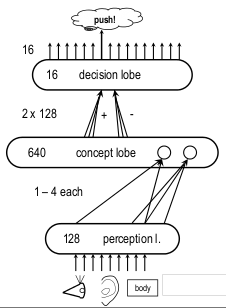
\includegraphics[width=4cm]{nornbrain.png}

{\tiny (Brom, 2006)}
\end{column}
\begin{column}{8cm}
\begin{itemize}
\item Mozek umělé bytosti ``Norn''
\item Perception: egg, toy, Norn, hunger, sexdrive
\item Concept: egg + hunger, Norn + sexdrive, \\ toy + egg + sexdrive
\item Decision: eat, mate, run, play
\only<1>{
\item Pomocný okruh pro Attention selection
\item Chceme podporovat užitečné koncepty a~vázat je na dobré akce
\item Náhodně inicializované váhy a~zpětná vazba!
\item Reinforcement záleží na změně {\em pudů} \\ (drives: hlad, sex, \dots)
}
\only<2>{
\item Suspectibility $\alpha$ a~průběžný reinforcement $r$
\item Vykonání akce zvýší $\alpha$ spojům po cestě, \\ to se s časem opět snižuje
\item Po snížení váhy k nule synapse migruje
\item Robustnost: Short-term weight, \\ long-term weight
}
\end{itemize}
\end{column}
\end{columns}
\end{frame}

\subsection{}
\begin{frame}{Otázky?}
\begin{center}
Příště UI: Reprezentace znalostí.

Příště Adaptivní agenti: Etologie a populační dynamika.
\end{center}
\end{frame}

\section{Neuronové sítě}

\subsection{}
\begin{frame}{Samoorganizace pomocí ANN}
\begin{itemize}
\item Umělé neurony (``výpočetní krabičky'') \\ dostávají vstupy (čísla) a na jejich \\ základě generují výstup (číslo)
\item Dnes: Chceme asociovat různé vstupy s různými neurony
\end{itemize}
\begin{tikzpicture}[remember picture,overlay]
  \node [xshift=-4.5cm,yshift=-4.5cm,above right] at (current page.north east)
    {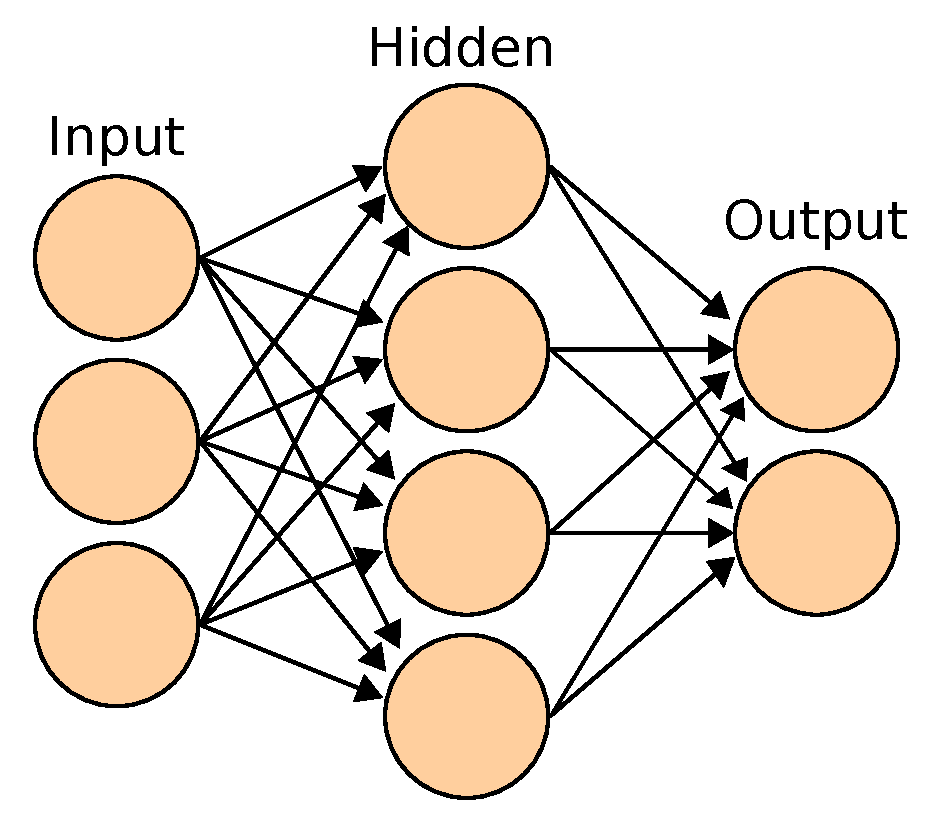
\includegraphics[width=4cm]{ANN.pdf}};
\end{tikzpicture}
\end{frame}

\subsection{}
\begin{frame}{Kohonenova mapa}
\begin{itemize}
\item Fonetický psací stroj, ekonomická data
\item Organizace, princip, učení
\item XXX: nebo jindy?!
\end{itemize}
\end{frame}

\subsection{}
\begin{frame}{Ojův algoritmus}
\begin{itemize}
\item PCA pomocí ANN
\end{itemize}
\end{frame}

\subsection{}
\begin{frame}{Další metody samoorganizace}
\begin{itemize}
\item Laterální inhibice, ART, RBF
\end{itemize}
\end{frame}

\subsection{}
\begin{frame}{Otázky?}
\begin{center}
Příště: ??
\end{center}
\end{frame}

\section{Datové struktury}

\subsection{}
\begin{frame}{Haldy}
\begin{itemize}
\item Rekapitulace.
\item Levicová halda.
\item Binomiální a Fibonacciho haldy.
\end{itemize}
\end{frame}

\subsection{}
\begin{frame}{B-stromy}
\begin{itemize}
\item Co to je, jak se to chová
\item Vlastnosti
\item Vyvažování
\end{itemize}
\end{frame}

\subsection{}
\begin{frame}{Otázky?}
\begin{center}
Příště: Datové struktury v externí paměti.
\end{center}
\end{frame}

\subsection{}
\begin{frame}{Děkuji vám}
\begin{center}
{\bf pasky@ucw.cz}

\vskip 6ex

Příště: Neuronové sítě.
	Adaptivní agenti.
	Evoluční algoritmy (koevoluce, otevřená evoluce, teoretická analýza). \\
	Složitost (vlastnosti tříd složitosti).
\end{center}
\end{frame}

\end{document}
